\documentclass{article}
\usepackage[margin=2cm]{geometry}
\usepackage{float}
\usepackage{graphicx}
\usepackage{lscape}
\usepackage{pdflscape}

% Paragraph settings
\setlength{\parskip}{10pt plus 1pt minus 1pt
\setlength{\parindent}{0cm}}

\begin{document}
\title{Design Description}
\author{Samuel Jackson \\ \texttt{slj11@aber.ac.uk}}
\date{\today}
\maketitle

\newpage
\begin{landscape}
\section{Class Diagram}

\begin{figure}[H]
\centering
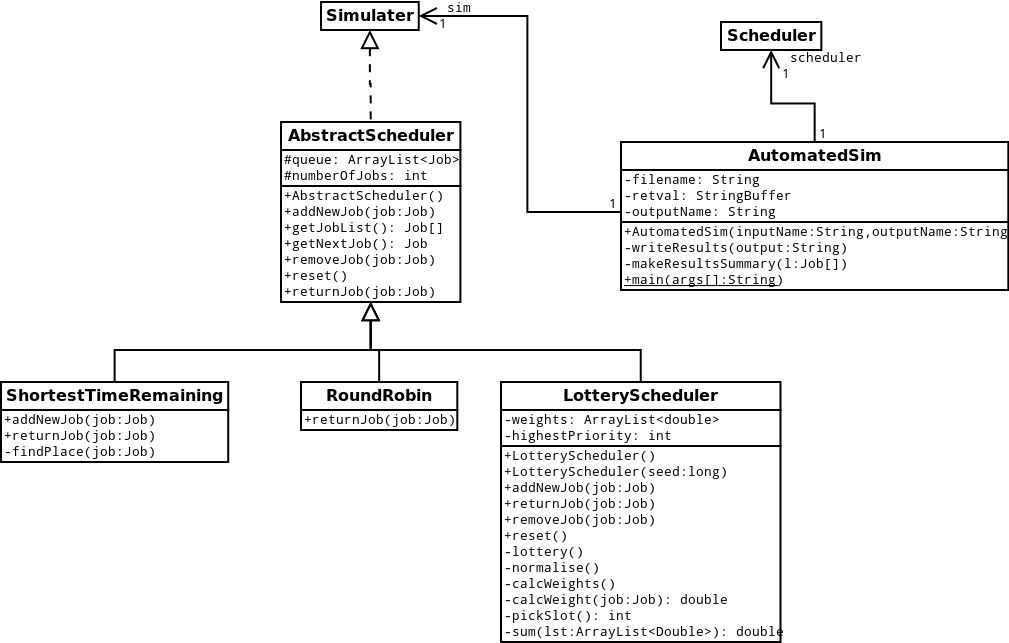
\includegraphics[width=1.1\textwidth]{class_diagram.png}
\caption{Class Diagram for the scheduling algorithms and automated simulator created for this project.}
\label{fig:class-diagram}
\end{figure}
\end{landscape}

\subsection{Description}
Figure \ref{fig:class-diagram} shows the class diagram for the classes that I have created for this project. Note that the $Simulator$, $Scheduler$ and $AbstractScheduler$ classes were not created by me and were provided with the existing system, but are shown here to illustrate how my classes extend from the current implementation. This diagram mainly documents the three additional scheduling algorithms I have implemented for this assignment; specifically shortest time remaining, round robin and weighted lottery scheduling. Additionally, the diagram also shows a fourth class called $AutomatedSim$ which was used for testing purposes. This section provides a brief description of each class.

\subsubsection{ShortestTimeRemaining}
$ShortestTimeRemaining$ contains the implementation of the shortest time remaining algorithm. This class overrides a couple of the methods inherited from the $AbstractScheduler$ class to add some implementation specific functionality and adds an additional method called $findPlace$. The $findPlace$ method calculates the amount of processing a job requires until it finishes and places in the queue according to this value with smaller remaining times being closer to the front. The $addNewJob$ method just calls $findPlace$, while $returnJob$ removes to job from its old position first and then re-inserts it to its new position using $findPlace$.

\subsubsection{RoundRobin}
The $RoundRobin$ class has the simplest implementation of the three scheduling algorithms. It overrides the $returnJob$ method by removing the returned job from the front of the queue and placing at the back.

\subsubsection{LotteryScheduler}
In contrast with $RoundRobin$, $LotteryScheduler$ has a much more complex implementation. $LotteryScheduler$ overrides four of the methods from $AbstractScheduler$. This is because a random lottery much be performed both when a job is returned to the queue and when a new job is added. The $removeJob$ method must also be overridden because the corresponding weight associated with a job must also be removed at the same time. For similar reasons the $reset$ method has also been overridden.

Additionally, this class also has several other methods to help with the running and maintenance of a random weighted lottery. The $lottery$ method selects a new job based on the weights and inserts it at the front of the queue. This method is called at both the $returnJob$ and $addNewJob$ methods. The $calcWeights$ method will iterate over each job in the queue and re-calculate the weight for the job based on its priority using the $calcWeight$ method. The $calcWeight$ method works on the basis that the lower the priority number, the greater importance the job has. The $highestPriority$ variable is used here to calculate the weighting. The $normalise$ method normalises the weights after a re-calculation to be within the range $0-1$. The $pickSlot$ method chooses a job based on the random weights and returns its index. Finally, $sum$ is a simple utility function to return the sum of all the numbers in an $ArrayList$
\end{document}